\documentclass{article}

\usepackage{minted}
\usepackage[most]{tcolorbox}
\usepackage{geometry}
\usepackage{enumitem}
\usepackage{hyperref}
\usepackage{hyperref}
\usepackage[parfill]{parskip}
\usepackage{wrapfig}
\usepackage{accsupp}

\geometry{margin=0.8in}
\definecolor{lightgreen}{rgb}{0.56, 0.93, 0.56}
\definecolor{moonstoneblue}{rgb}{0.45, 0.66, 0.76}
\definecolor{magenta}{rgb}{0.8,0.66,0.76}
\begin{document}
\BeginAccSupp{}
\begin{flushright}
Computational Biology ~\\
Tufts University Bio 35 ~\\
Fall 2021 ~\\ ~\\
\end{flushright}
\begin{center}{\textbf{\Large{Spotlight 11: Pleuni Pennings}}}\end{center}

\textit{Please note that in general I have taken/adapted the words of our Spotlight subjects from their own websites to describe their work. I have done this in an effort to maintain accuracy in describing their research programs. Please do not copy paste text from their papers/websites in your assignments!}

\begin{wrapfigure}{L}{0.08\textwidth}
\begin{center}
 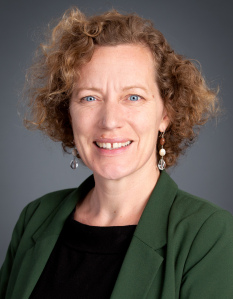
\includegraphics[width=0.09\textwidth]{images/pleuni-pennings.jpeg}
 \end{center}
\end{wrapfigure}
~\\ As part of our unit on viral evolution, we will explore the work of Pleuni Pennings. Prof. Pennings is an evolutionary biologist and works on the evolution of drug resistance in HIV. She wants to understand what determines the rate of evolution of drug resistance, so that we can find ways to halt the evolution of drug resistance. Her work has also been very influential in modeling the genetic mechanisms underlying rapid adaptation. Dr. Pennings is a Professor at San Francisco State University.
~\\ 

Please read the following article about HIV evolution and drug resistance by Prof. Pennings: 
\begin{enumerate}
\item \texttt{\href{https://www.mdpi.com/2036-7449/5/11/s1.e5}{https://www.mdpi.com/2036-7449/5/11/s1.e5}}
\end{enumerate}

Also watch to the following video by her collaborator Prof. Alison Feder about their joint work on HIV evolution:
\begin{enumerate}
\item \texttt{\href{https://youtu.be/43M55F_g9zM}{https://youtu.be/43M55F\_g9zM}}
\end{enumerate}

\subsubsection*{Written Assignment} 
After reading Pleuni Pennings's articles and watching the video, write a reflection (max one page) on what you discovered. You might wish to address some of the following: 

\begin{enumerate}
\item What was most interesting to you in reviewing these resources?
\item What did you learn from these resources about the evolution of drug resistance? How could a better understanding of drug resistance evolution help us design better drugs, and how might computational tools be useful in this pursuit?
\item What new questions do you have after reviewing these resources?
\item What do these resources tell you about the types of people that do computational biology, or their motivations?
\end{enumerate}
\EndAccSupp{}

\end{document}